\chapter{Derivatives}\label{ch:derivatives}
%\epigraph{Some people will tell you that slow is good---but I'm here to tell you that fast is better.}{Hunter S. Thompson}%, Kingdom of Fear: Loathsome Secrets of a Star-crossed Child in the Final Days of the American Century}

Say we are trying to find the rate of change of the function $x^3$.
That is, essentially, its slope.
\begin{figure}[H]
  \begin{center}
    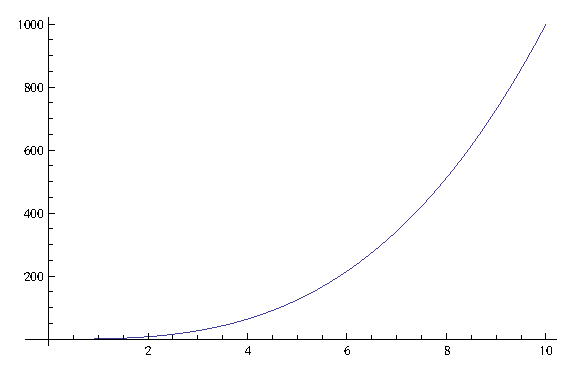
\includegraphics[width=0.5\textwidth]{continuous/derivatives/x3.eps}
  \end{center}
  \caption{A plot of $x^3$.}
\end{figure}
We'd like to be able to do this with just a straight line, but that's simply not possible.
We could, however, draw a straight line that approximates this function around a specific value, say $x=1$.
We can just draw a line that approximates the function, to try to get it right:
\begin{figure}[H]
  \begin{center}
    \includegraphics[width=0.5\textwidth]{continuous/derivatives/x3_1.eps}
  \end{center}
\end{figure}
But that's not a very accurate impression of our slope.
To make it better, we could draw a line between two points that are \emph{even closer} to $x=1$.
\begin{figure}[H]
  \begin{center}
    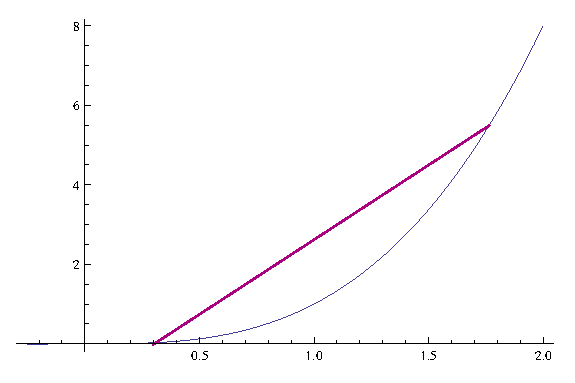
\includegraphics[width=0.5\textwidth]{continuous/derivatives/x3_2.eps}
  \end{center}
\end{figure}
And to improve this further, we can continue to draw lines closer and closer to that point.
\begin{figure}[H]
  \begin{center}
    \includegraphics[width=0.5\textwidth]{continuous/derivatives/x3_3.eps}
  \end{center}
\end{figure}
\begin{figure}[H]
  \begin{center}
    \includegraphics[width=0.5\textwidth]{continuous/derivatives/x3_4.eps}
  \end{center}
\end{figure}
Until we are drawing lines between two points which are an \emph{infinitely small} distance apart from one another.
\begin{figure}[H]
  \begin{center}
    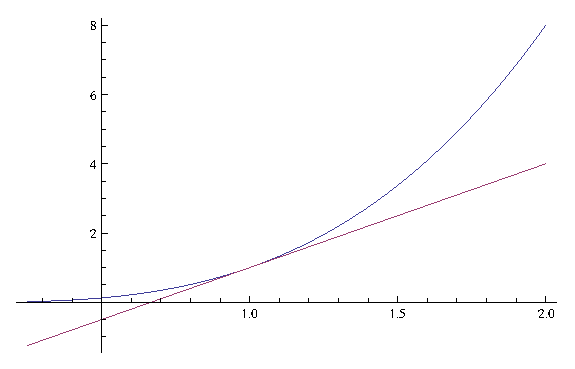
\includegraphics[width=0.5\textwidth]{continuous/derivatives/x3vline.eps}
  \end{center}
  %\caption{A plot of $x^3$ and $3x-2$.}
\end{figure}
The slope of this line is the \emph{derivative\/} of our function at $x=1$.

We see that, around $x=1$, our slopes are very close.
But as we get further from that $x$-value, we don't have a very good approximation of the slope anymore.
This is because a derivative describes the {\em instantaneous rate of change\/} of the function \emph{at that point}.
It's not the slope of the entire function, it's just the slope at one, specific, selected point.

The \textbf{derivative}\index{derivative} of a function $f(x)$ at $x=a$ is used to describe its \emph{instantaneous slope} at the value $x=a$.

\section{Slopes}
\index{slope}
The entire idea of a derivative is based on the idea behind the slope of a graph.
\begin{figure}[H]
  \begin{center}
    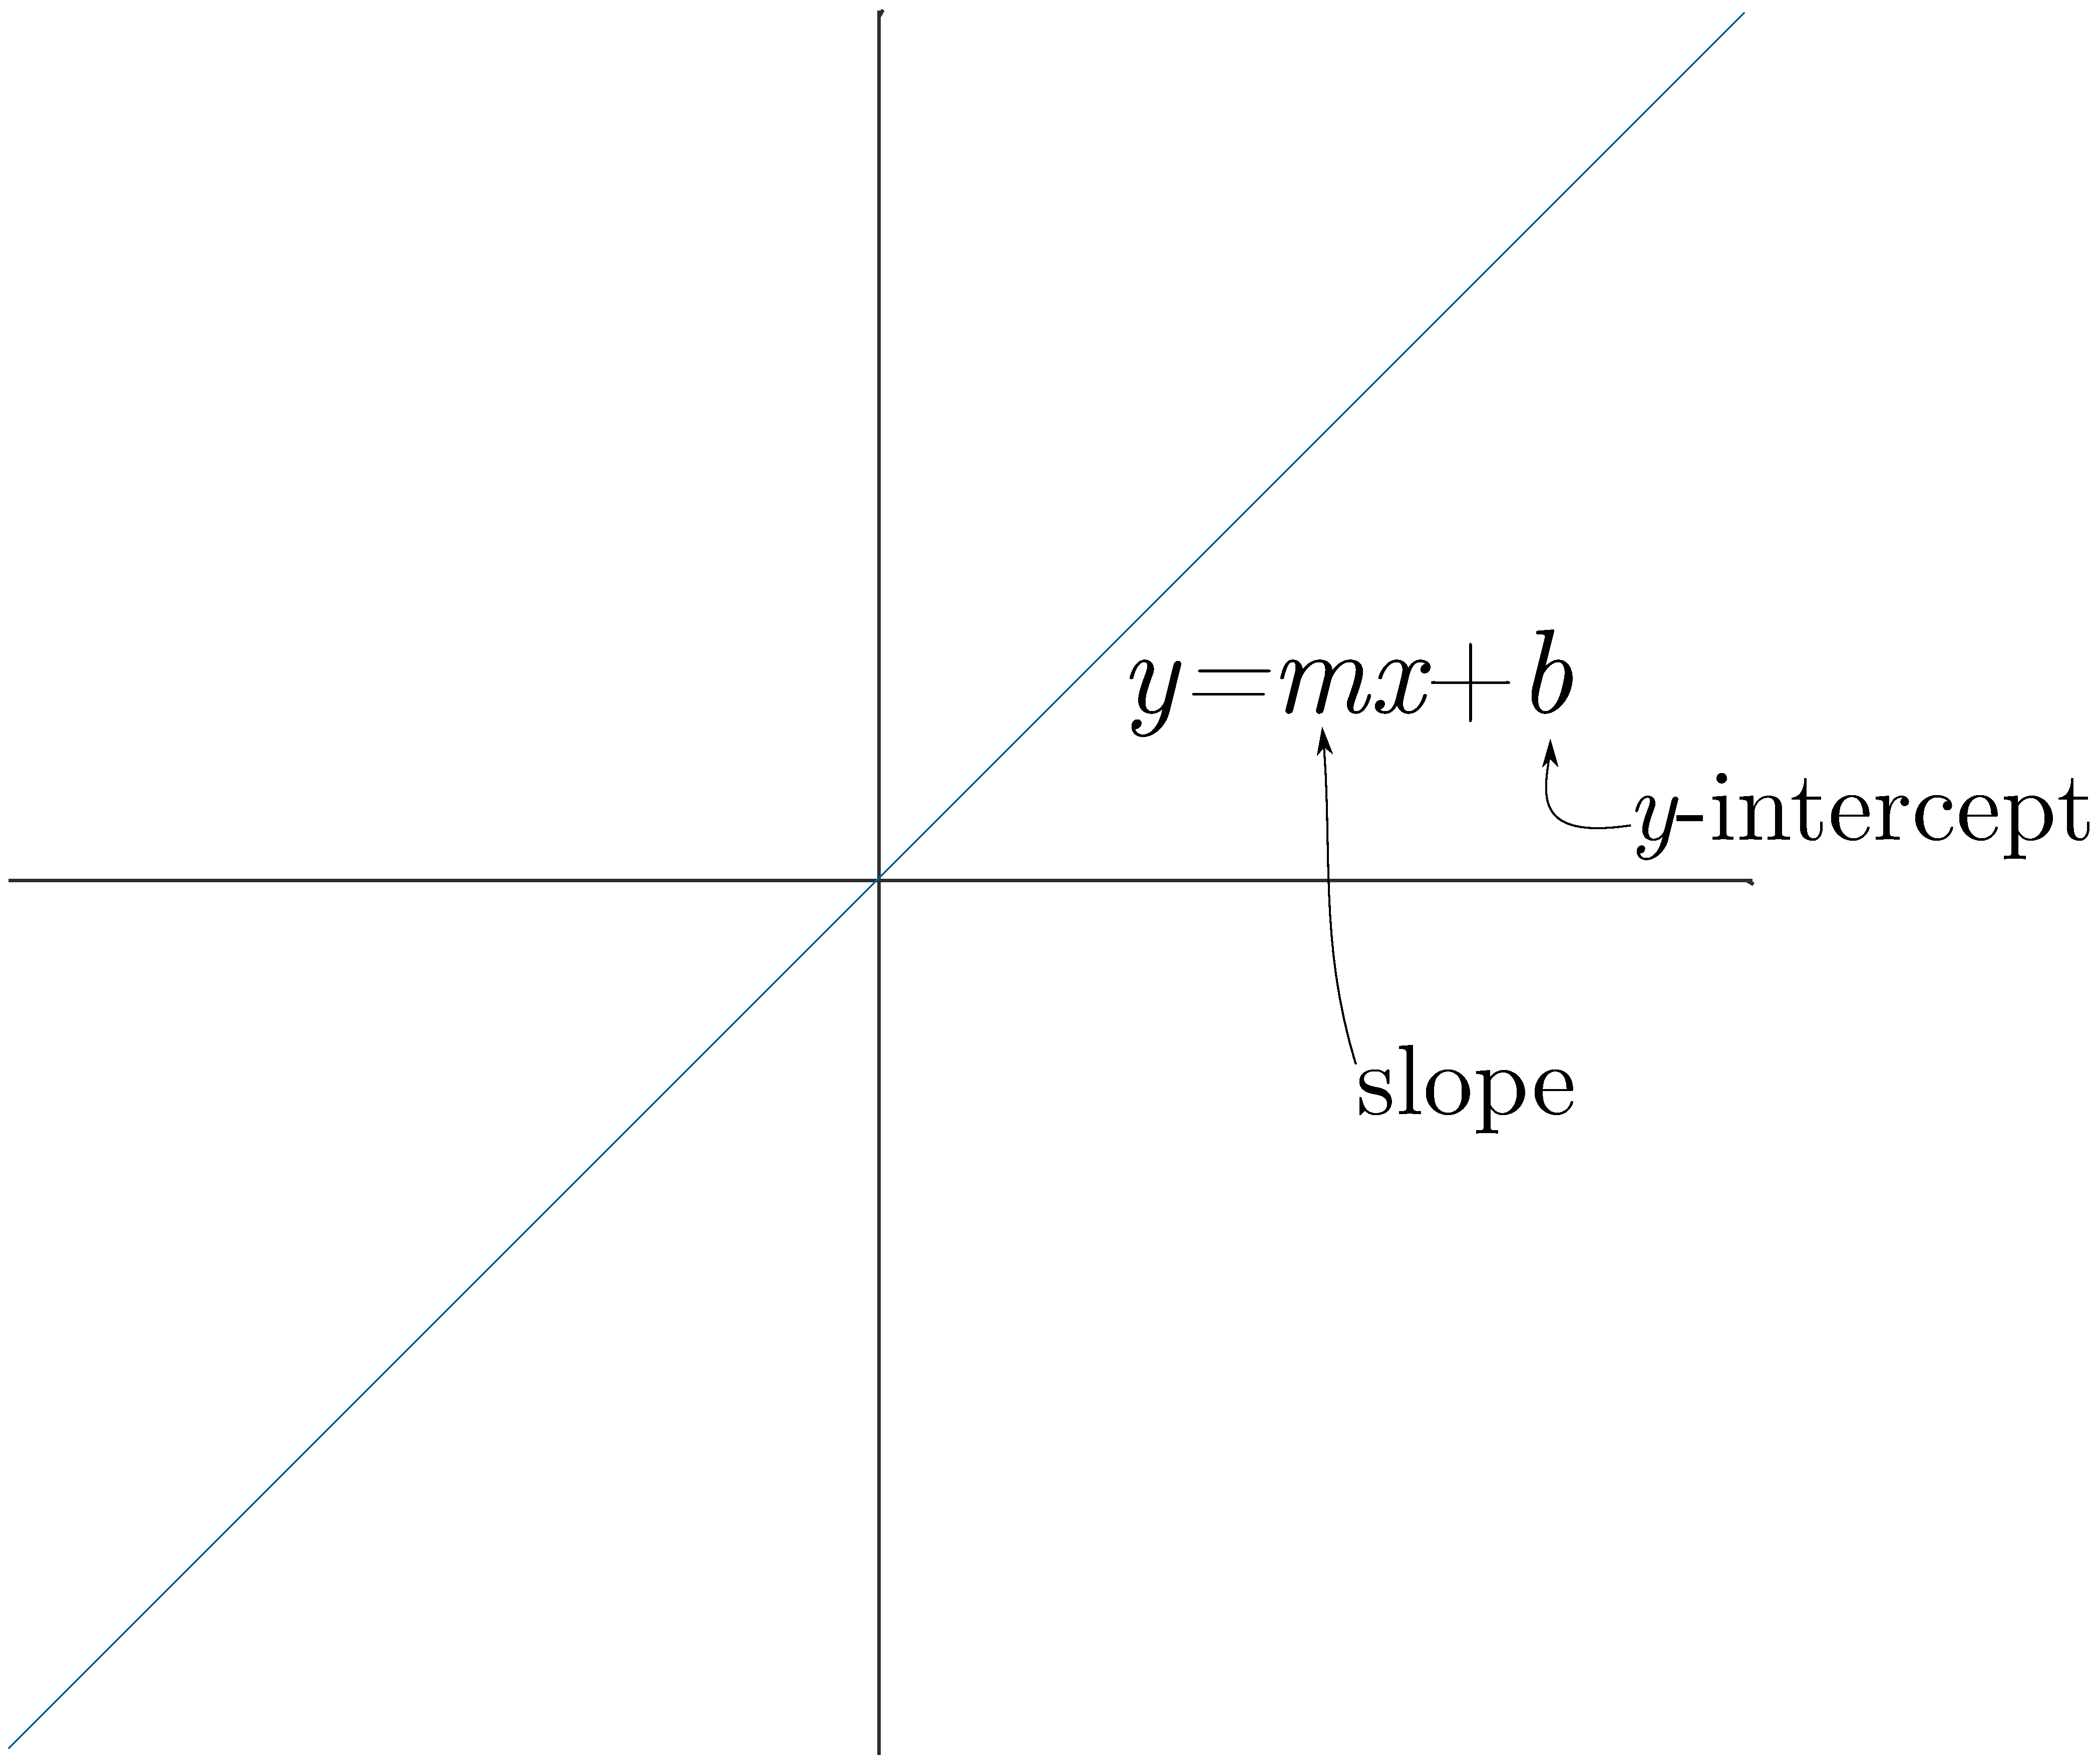
\includegraphics[width=0.5\textwidth]{continuous/derivatives/lineform.eps}
  \end{center}
  \caption{The slope-intercept form equation for a line.}
  % Kyle Martin corrected this caption for me. Thanks Kyle!
\end{figure}
The slope, $m$, of a given straight line\footnote{$b$ is the $y$-{\em intercept} of the function.}
$f(x)=mx+b$ is given by its \emph{change in $y$ values divided by its change in $x$ values}
\begin{align}
  \label{eq:slope}
  m&=\frac{\Delta y}{\Delta x,} \\
  \intertext{which we can find using the formula}
  m&=\frac{y_2-y_1}{x_2-x_1,} \\
  \intertext{which is equivalent to}
  m&=\frac{f(x_2)-f(x_1)}{x_2-x_1.}
\end{align}
\begin{figure}[H]
  \begin{center}
    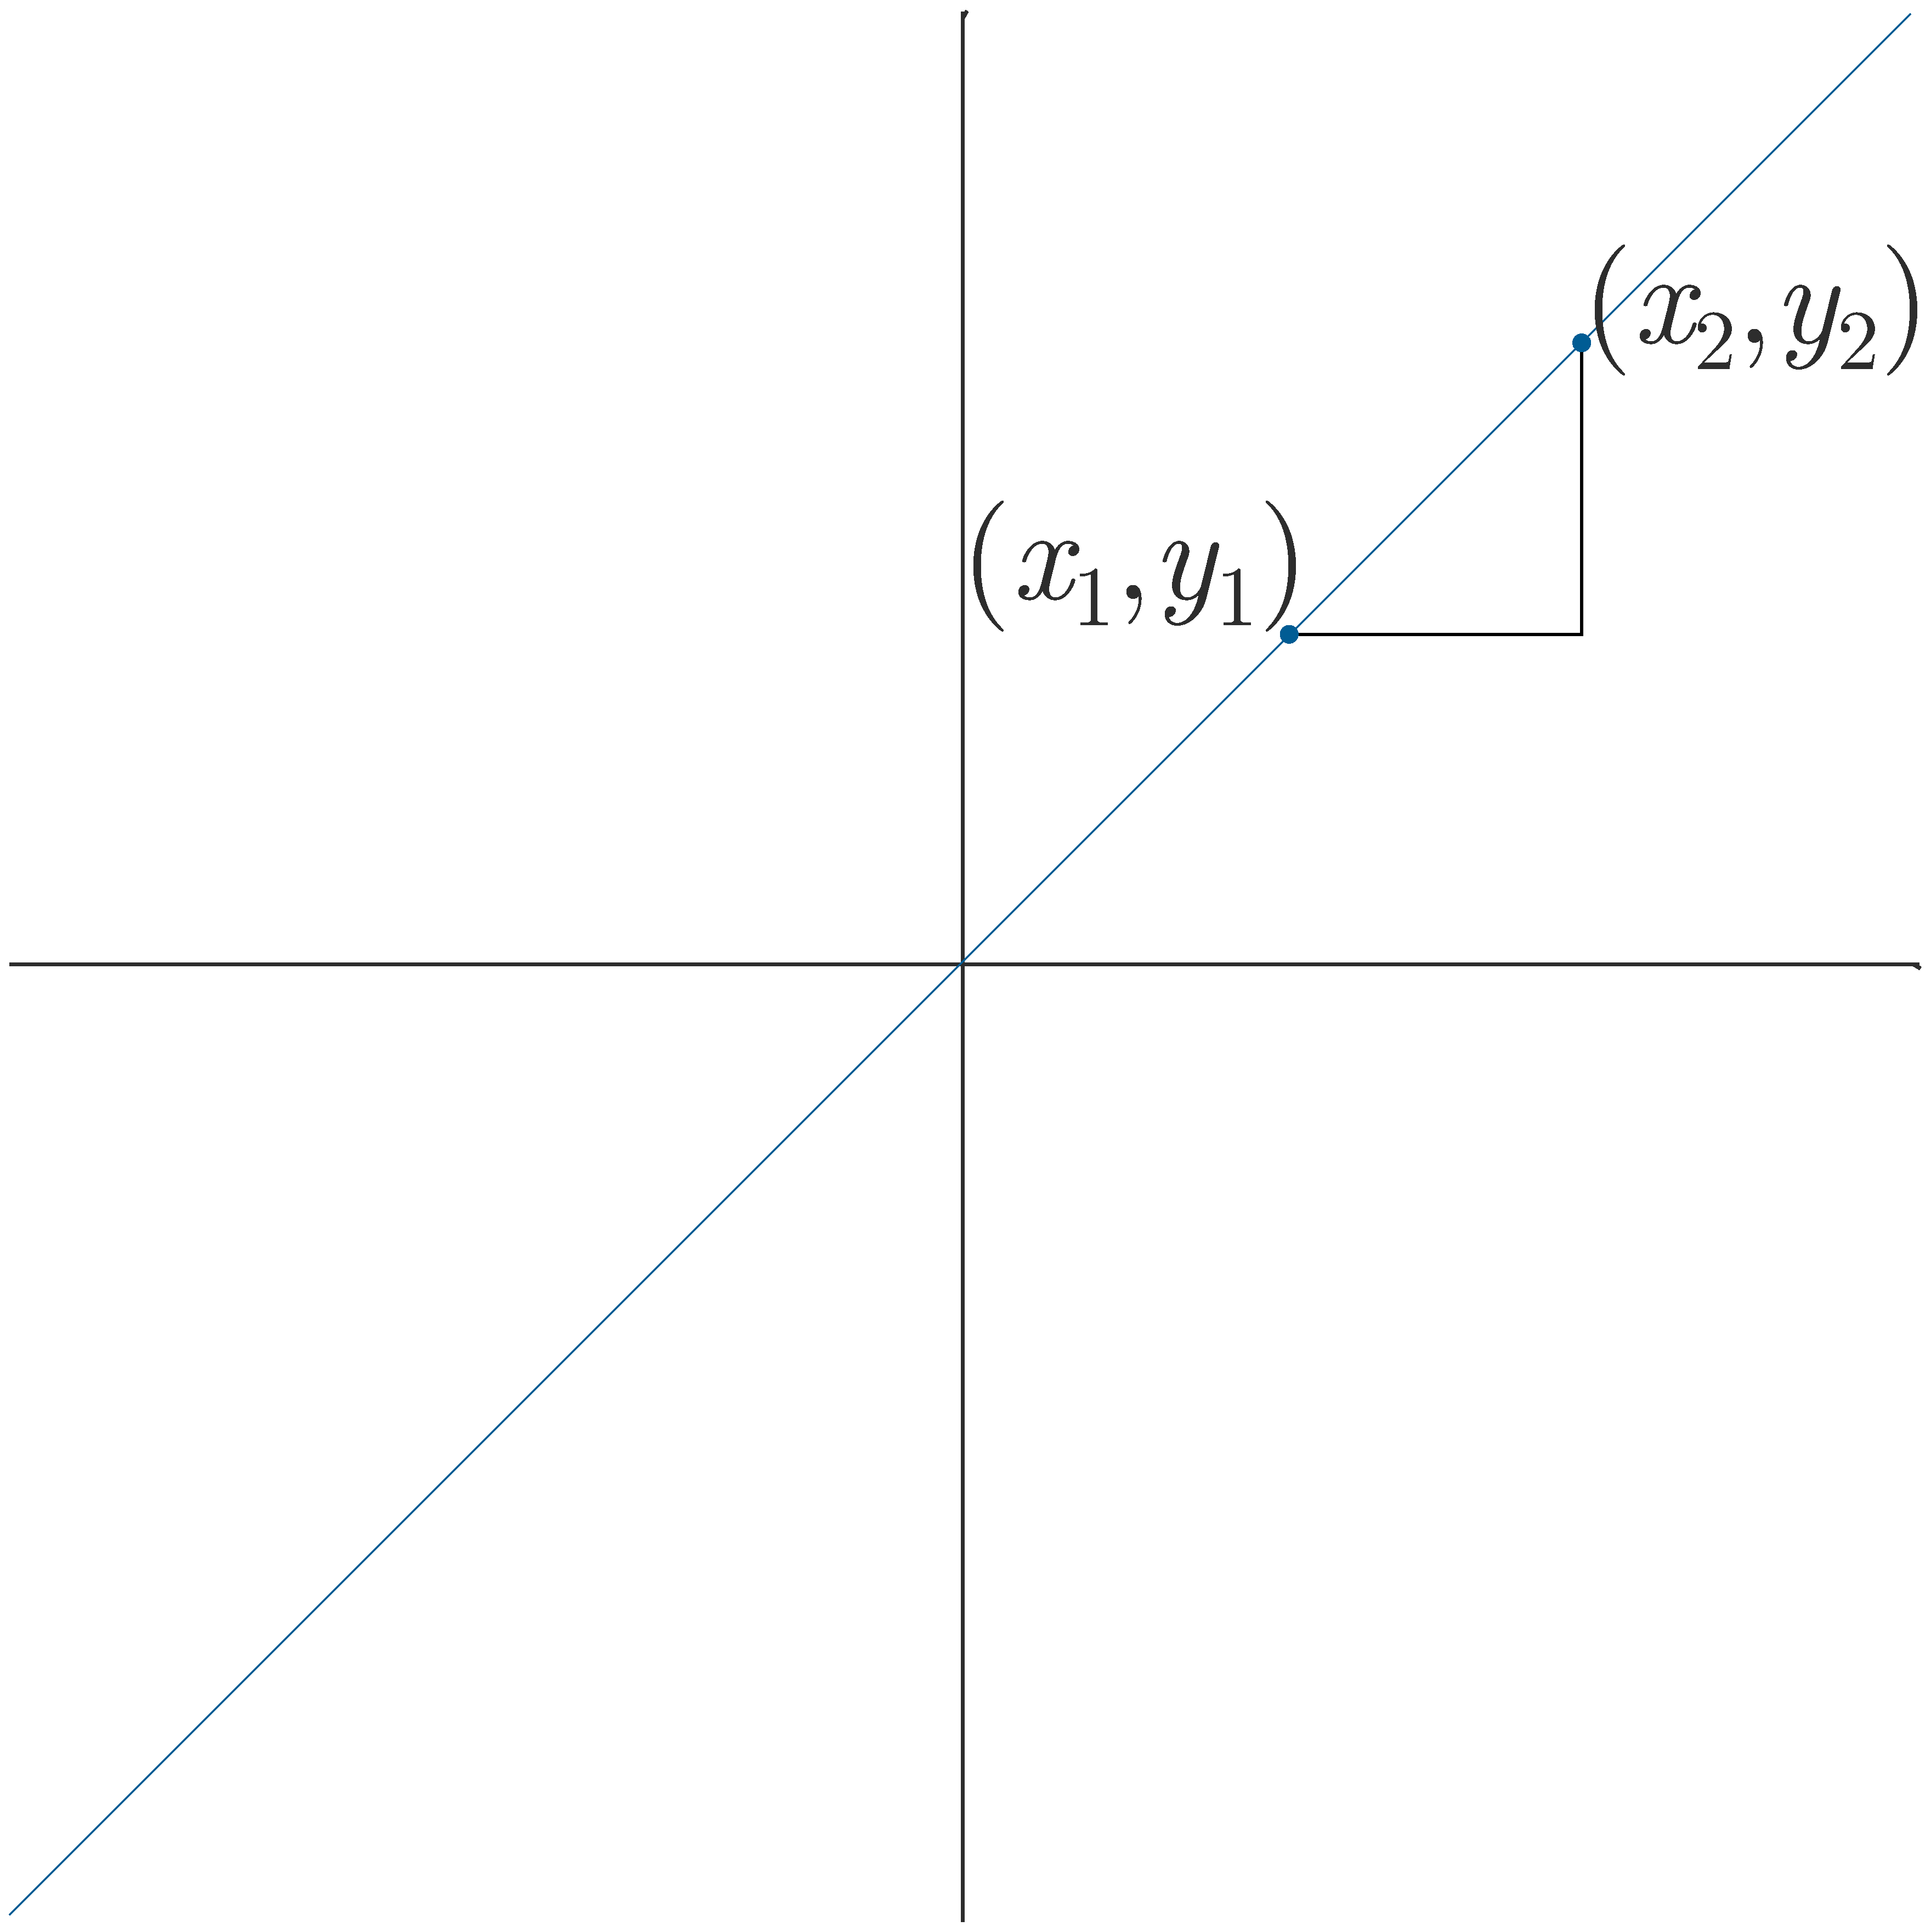
\includegraphics[width=0.5\textwidth]{continuous/derivatives/lineform_slope.eps}
  \end{center}
  \caption{How we determine slope in a graph.}
\end{figure}
% In early mathematics courses, slope is often described as the ``rise'' over ``run'' of a graph.
% While this is accurate, it doesn't provide the complete picture.
% What a \emph{slope} really describes is how much a given function $f(x)$ is altering each of its input values $x$, often heard as ``change in $y$ over change in $x$.''
% You'll notice that this is independent of any initial value $b$ selected for a linear function.\footnote{Which is why all constants disappear when you take the derivative of a function.}

\section{The Difference Quotient}\index{difference quotient}

The \emph{difference quotient} works the same way as the slope formula, except we treat how far apart our two $x$ values are as a variable.
\begin{equation}
  \frac{\Delta f(x)}{\Delta x}=\frac{f(x+\Delta x)-f(x)}{\Delta x}
\end{equation}
So $\Delta x=x_2-x_1$, and $x=x_1$.
\begin{figure}[H]
  \begin{center}
    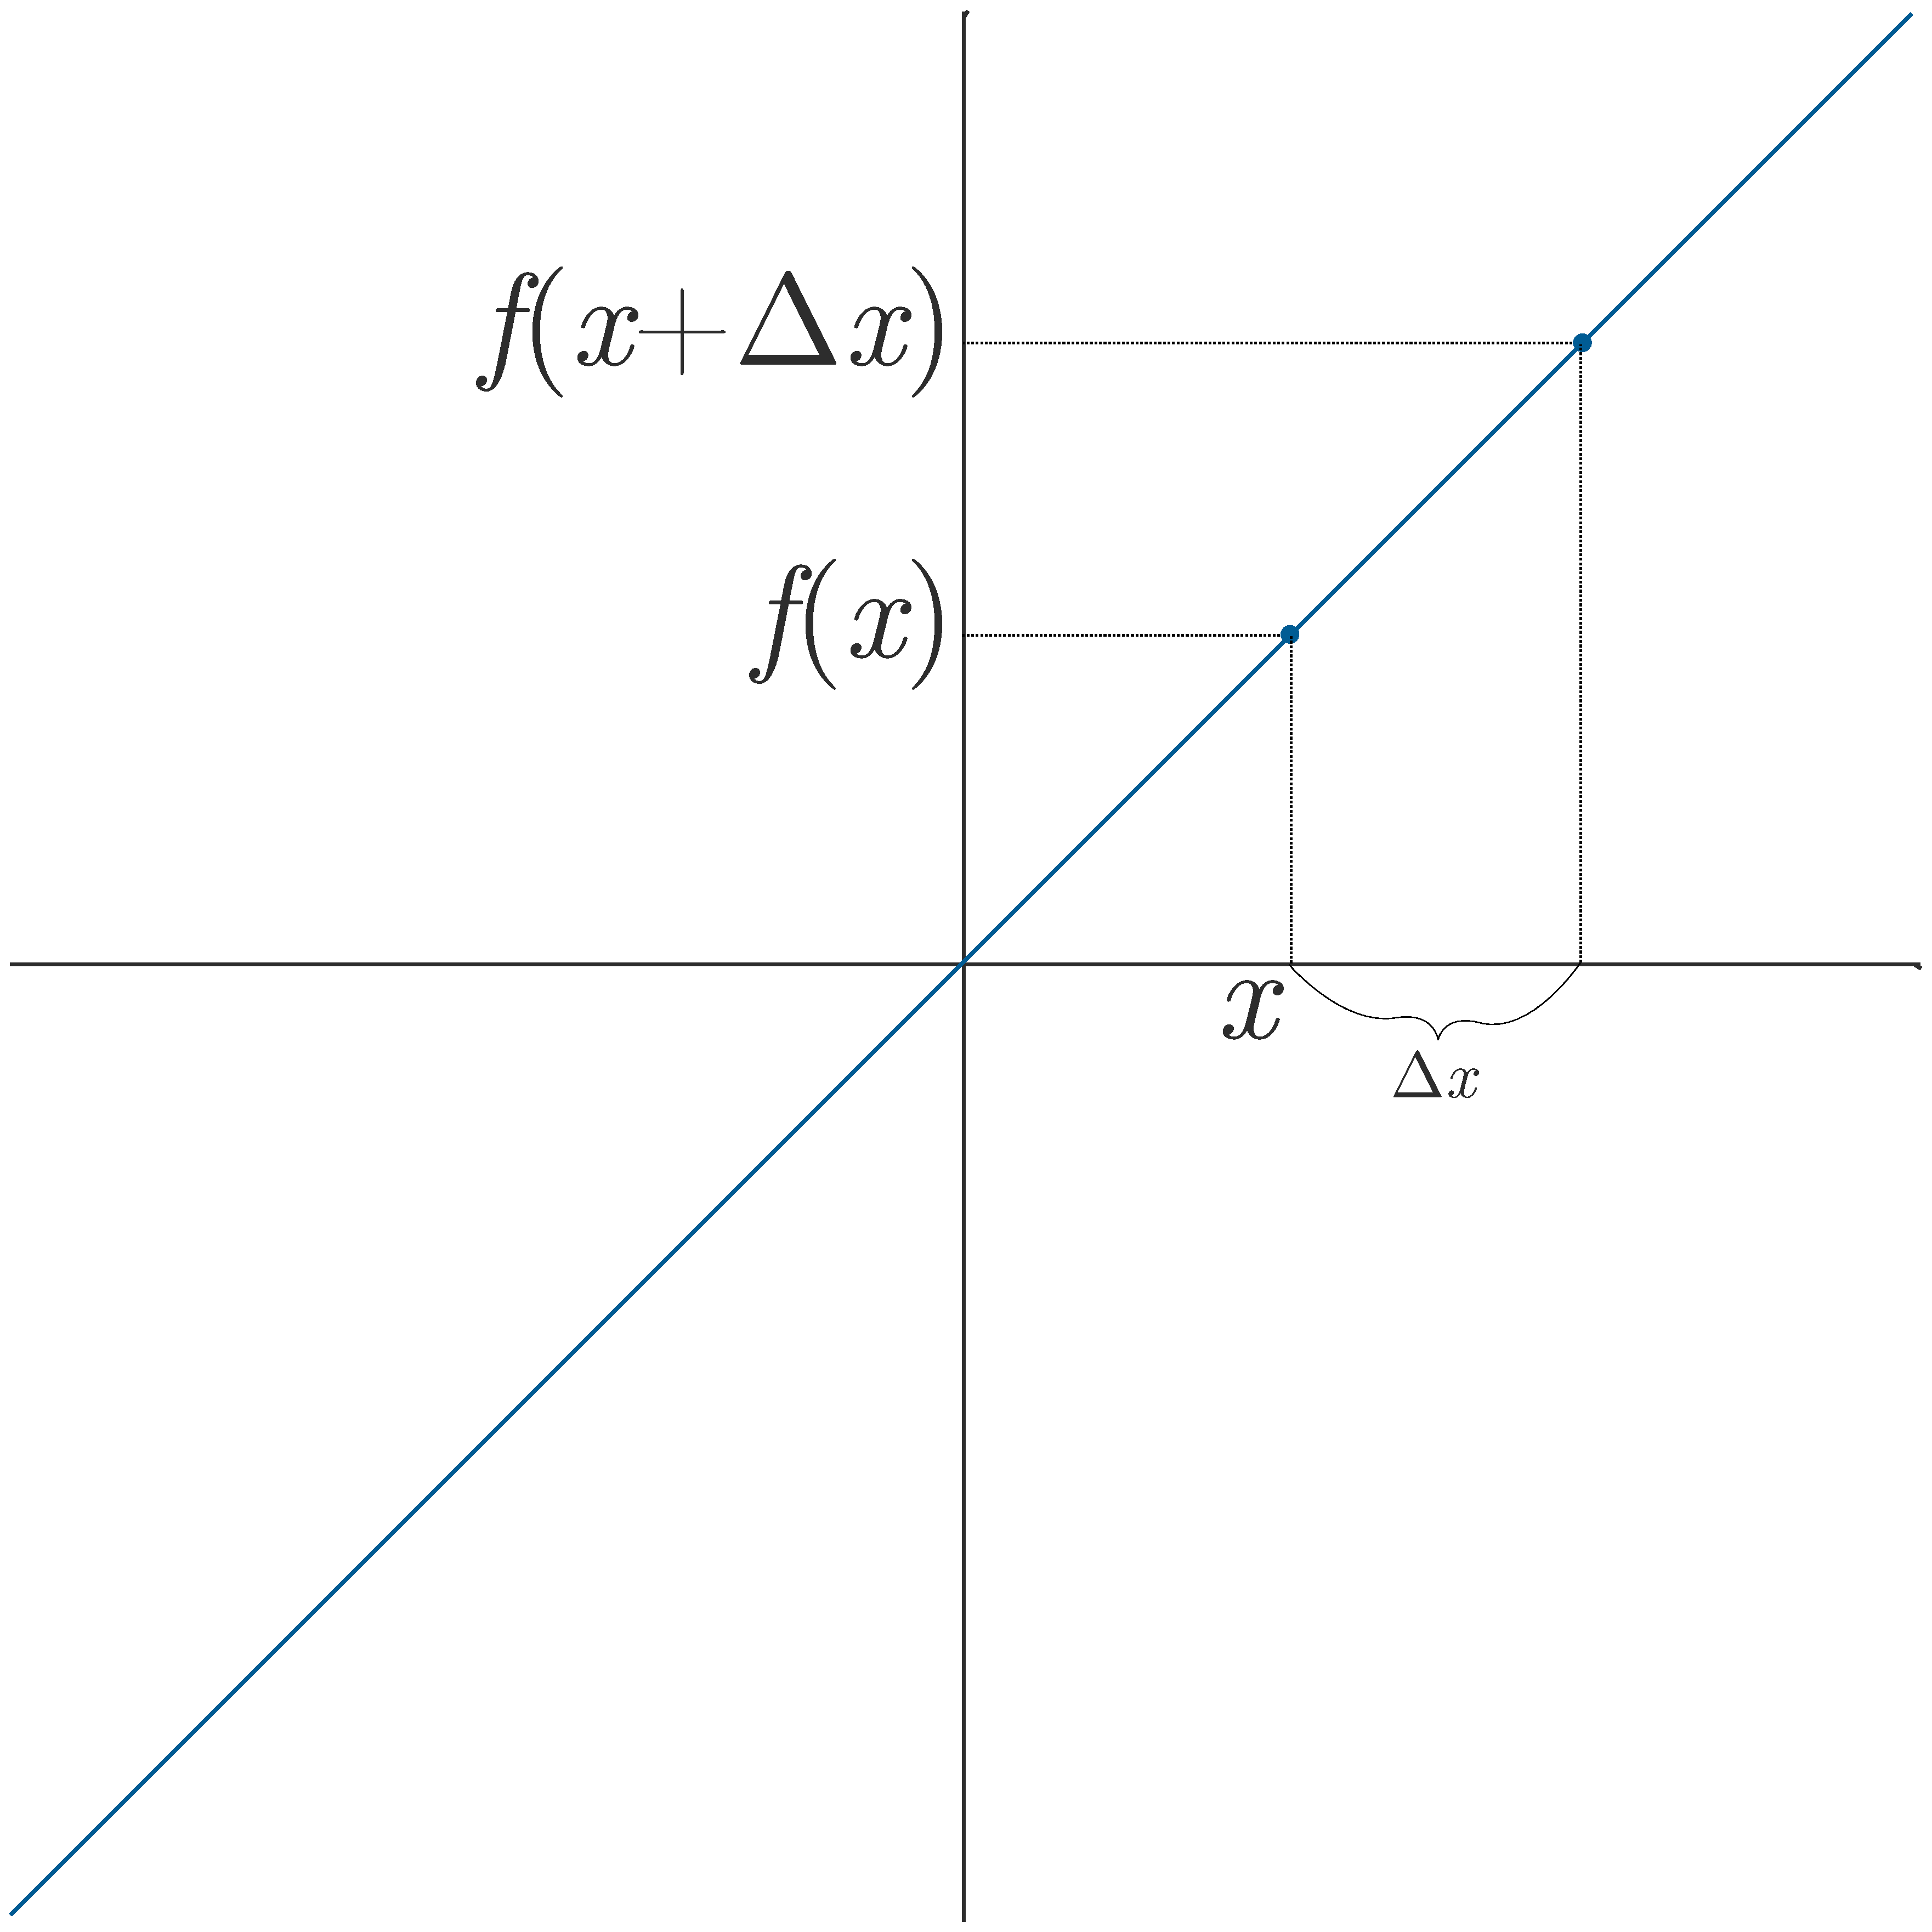
\includegraphics[width=0.5\textwidth]{continuous/derivatives/diffquot.eps}
  \end{center}
  \caption{A visual representation of the difference quotient on a line.}
\end{figure}
You'll often see the difference quotient written with $\Delta x \to h$ as
\begin{equation}
  \frac{\Delta f(x)}{\Delta x}=\frac{f(x+h)-f(x)}{h}
\end{equation}

\subsection{Limit Definition of Derivatives}

The difference quotient is used in the \textbf{limit definition of a derivative}\index{derivative, limit definition}, which is
\begin{equation}
  \label{eq:limitdef}
  \frac{\ud f(x)}{\ud x}=\lim_{h \to 0} \frac{f(x+h)-f(x)}{h}
\end{equation}
% Notice that the only distinction between this equation and the difference quotient/slope equation from earlier is the introduction of a limit. The idea behind that limit is that you're calculating the slope of a function as the distance between your $x_2$ and $x_1$ values becomes infinitely small ($h\to 0$). We call this distance an \emph{infinitesimal}: a distance smaller than any feasible measurement, but not zero in size.
%
% So what a derivative of a function is going to tell us is how the function behaves (its slope) at a particular ``infinitely small'' portion of the graph, which might as well be a point.
%
% For linear functions, the function behaves the same no matter where you look at it, so their derivatives are always constant and equal to the slope of the function.
%
% For nonlinear functions, like $f(x)=x^2$, the derivative will yield a function (in this case, just $f'(x)=2x$), because the function is changing its input values differently depending on where you are looking. Near the origin, where $x=0$, the derivative is zero and any $x$ value will give $y$ values not too far from the original input. But as you move further from the origin, the ratio of $y/x$ gets larger and larger, and the derivative in turn gets bigger and bigger.
% \begin{figure}[H]
%     \begin{center}
%       \includegraphics[width=0.5\textwidth]{continuous/derivatives/xsquared.eps}
%       \caption{A graph of $f(x)=x^2$ and $f'(x)=2x$.}
%     \end{center}
% \end{figure}

\section{Notation Used with Derivatives}

There are a number of ways to denote the derivative of a function $y=f(x)$. The most common notation early on in calculus classes is the \emph{prime} notation $y'$ and $f'$ because it is the simplest. Later on, you often see $\ud/\ud x$ style notation, because it is more specific. It tells us not only which function we are differentiating, but with respect to which variable. A notable characteristic of this ``d notation'' is the similarity it provides to our equation for slope:
\begin{align*}
  &m=\frac{\Delta y}{\Delta x}=\frac{\Delta f(x)}{\Delta x} &y'=\frac{\ud y}{\ud x}=\frac{\ud f(x)}{\ud x}
\end{align*}
In the case of slope, we're talking about specific $y$ and $x$ values, but in the case of a derivative, we're talking about \emph{infinitesimals}, and that particular distinction allows us to discuss the behavior of functions that aren't linear, but change their behavior over time.

\section{Tangent Lines}

Remember our line that gave us the slope of $f(x)=x^3$ at $x=1$?
That was called a \emph{tangent line} to $f(x)$ at that point.
How do we find out what the equation for that line is?

Well, we use the derivative of the function, calculated at $x=1$, to determine the slope of our tangent line.
\begin{align*}
  f(x)&=x^3\\
  f'(x)&=\lim_{h \to 0} \frac{f(x+h)-f(x)}{h} \\
  \intertext{Remembering back to Section \ref{sec:compositefunctions},}
  f'(x)&=\lim_{h \to 0} \frac{(x+h)^3-x^3}{h} \\
  \intertext{Expand $(x+h)^3$.}
  f'(x)&=\lim_{h \to 0} \frac{(x+h)(x+h)(x+h)-x^3}{h} \\
  f'(x)&=\lim_{h \to 0} \frac{(x^2+hx+hx+h^2)(x+h)}{h} \\
  f'(x)&=\lim_{h \to 0} \frac{(x^2+2hx+h^2)(x+h)}{h} \\
  f'(x)&=\lim_{h \to 0} \frac{x^3+2hx^2+h^2x+x^2h+2h^2x+h^3-x^3}{h} \\
  f'(x)&=\lim_{h \to 0} \frac{3hx^2+3h^2x+h^3}{h} \\
  f'(x)&=\lim_{h \to 0} 3x^2+3hx+h^2 \\
  \intertext{Since we are taking the limit as $h\to0$,}
  f'(x)&=3x^2
\end{align*}
If we calculate this derivative at $x=1$, we get
\begin{align*}
  f'(x)\Big|_{x=1}&=3(1)^2 \\
  &=3
\end{align*}
So the slope of our tangent line is $3$.
\begin{note}
  The symbol $\big|_{x=1}$ means to evaluate the preceding term at the value $x=a$.
  It is often seen referring to a function's derivative at a particular point, which is different from the function's derivative in general.
\end{note}

Now we use the point-slope formula (Section \ref{sec:pointslope}) with $m=3$ to find the equation for our tangent line.
\begin{align*}
  y-y_1 &= m (x-x_1) \\
  y &= mx-mx_1 +y_1 \\
  y&=3x-3\cdot 1 + 1 \\
  y&=3x-2
\end{align*}
Which tells us that the equation for the tangent line to our function at $x=1$ is $y=3x-2$.
\begin{figure}[H]
  \begin{center}
    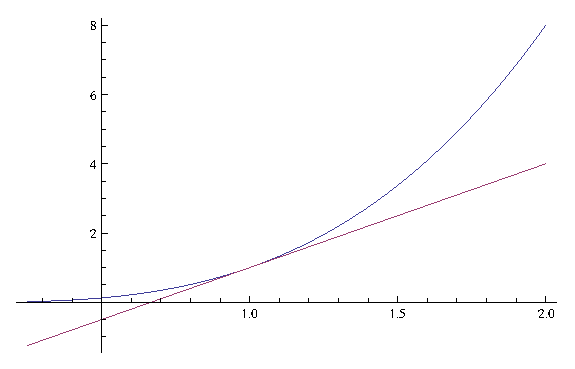
\includegraphics[width=0.5\textwidth]{continuous/derivatives/x3vline.eps}
  \end{center}
  \caption{A plot of $x^3$ and $3x-2$.}
\end{figure}
\subsection{Derivative Rules}
But that was an awful lot of work just to get one little derivative!
It would be handy if we could generalize the derivative of functions like this, so that we don't have to do it again in the future.
Luckily, we can, and this generalization is what we call the \emph{power rule}.

The \textbf{power rule}\index{power rule} states that
\begin{equation}
  \ddx x^n=nx^{n-1}
\end{equation}

\begin{ex}
  Find the derivative of $f(x)=x^9$ with respect to $x$.
  \begin{sol}
    We subtract $1$ from the value of our exponent and make the original exponent the coefficient of the variable.
    This means that
    \[ \frac{\ud f(x)}{\ud x} = 9x^8. \]
  \end{sol}
\end{ex}
\begin{ex}
  The power rule also works for negative exponents.
  Let's try finding the derivative of $f(x)=\frac{1}{x}$ with respect to x.
  \begin{sol}
    To find this derivative, we first recognize that $x^{-1} \equiv 1/x$.
    \begin{align*}
      f(x)&=\frac{1}{x}=x^{-1}
      \intertext{And now simply use the power rule as normal.}
      f'(x) &= -1 \cdot x^{-2} \\
      \intertext{Simplify.}
      f'(x)&= -\frac{1}{x^2}
    \end{align*}
  \end{sol}
\end{ex}

% The \emph{tangent line} to a graph at a point is just a line that acts like the function is linear and behaves exactly as the graph does at that point. This is useful for visualizing the derivative, and showing us how the behavior of a function can change depending on its $(x,y)$ location.

% \begin{figure}[H]
%   \begin{center}
%     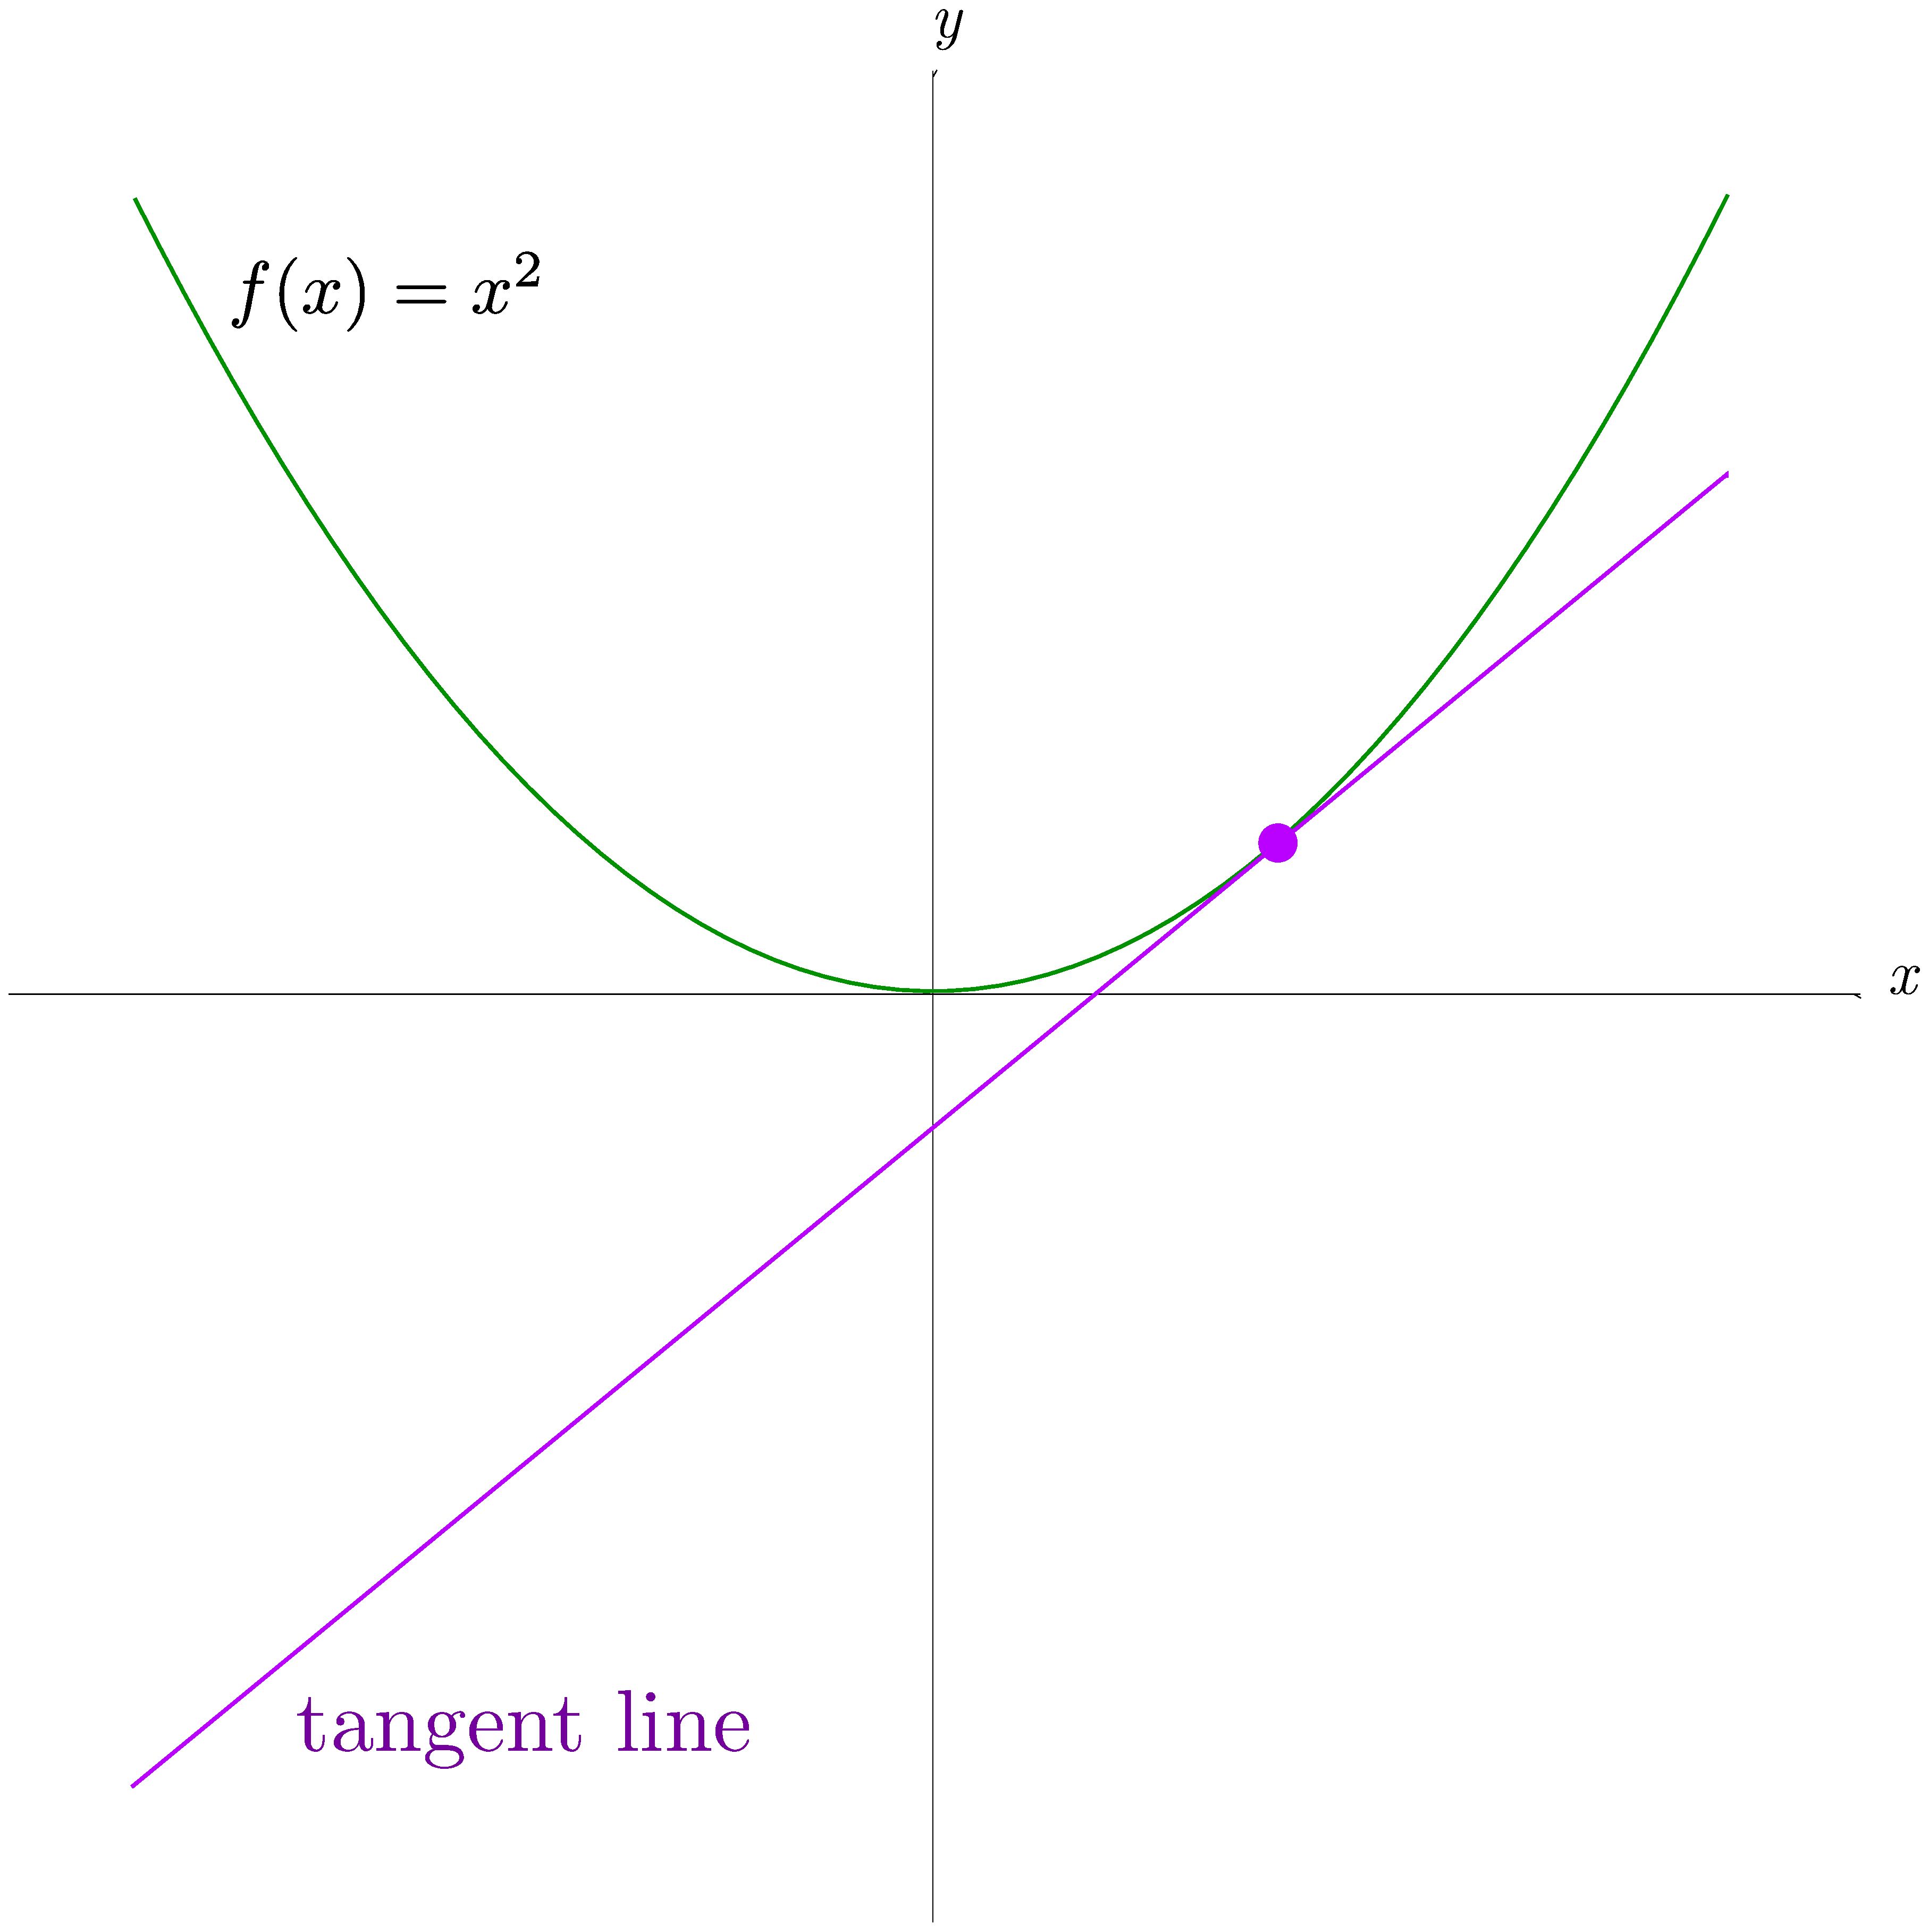
\includegraphics[width=0.4\textwidth]{continuous/derivatives/tangent.eps}
%   \end{center}
%   \caption{A tangent line to the graph of $f(x)=x^2$.}
% \end{figure}
%
% To calculate the equation for a tangent line at a point, simply find the
% derivative of the function at that point and treat that as the slope of the
% tangent line. Then, use the $(x, y)$ values of the point to produce the tangent line's function
% using the point-slope equation (\eqref{eq:pointslope}).

Derivative rules are just shorthands for working things out manually using the limit definition in equation \eqref{eq:limitdef}.
They all come from equation \eqref{eq:limitdef} and greatly simplify the work we have to do in calculating derivatives.

Before we go further, let's cover some important properties to know when finding derivatives.
First, the \emph{derivative of a sum} is the same as a \emph{sum of derivatives}.
\begin{theorem}[Sum Rule for Derivatives]
  For two differentiable functions $u(x)$ and $v(x)$,
  \[ \ddx [u(x)+v(x)] = \ddx u(x) + \ddx g(x). \]
  \label{th:sumrulederiv}
  \begin{proof}
    Start with the limit definition of a derivative.
    \begin{align*}
      \ddx \big[u(x)+v(x)\big] &= \lim_{h\to\infty} \frac{\big[u(x+h)+v(x+h)\big]-\big[u(x)-v(x)\big]}{h} \\
      &= \lim_{h\to\infty} \frac{u(x+h)-u(x)+v(x+h)-v(x)}{h} \\
      &= \lim_{h\to\infty} \frac{u(x+h)-u(x)}{h} + \lim_{h\to\infty} \frac{v(x+h)-v(x)}{h}\\
      &= \ddx u(x) + \ddx v(x) \qedhere
    \end{align*}
  \end{proof}
\end{theorem}
\index{derivatives, sum of}
\begin{ex}
  Find the derivative of $f(x)=x^2+x$.
  \begin{sol}
    We now know that
    \[ f'(x) = \ddx (x^2+x)\]
    is equivalent to
    \[ f'(x) =\ddx x^2 + \ddx x.\]
    Simply use the power rule to differentiate.
    \begin{align*}
      f'(x) &= 2x+1\cdot x^0 \\
      \intertext{Since any number raised to the power $0$ is just $1$,}
      f'(x)&= 2x+1.
    \end{align*}
  \end{sol}
\end{ex}

When differentiating functions involving constant multiples, we may move the constants out of the derivative.
This means that, if $g(x)$ is a differentiable function and $k$ is a constant multiple,
\[ \ddx \big( k g(x) \big) = k \ddx \big(g(x)\big).\]
This is known as the \textbf{constant multiple rule}.\index{derivatives, constant multiples}

The derivate of a constant is always zero, because constant has no rate of change.
\begin{theorem}[Constant Rule for Derivatives]
  For any constant number $k$, we know that
  \[\ddx k=0.\]
  \label{th:deriv:constantrule}
\end{theorem}
This is called the \textbf{constant rule for derivatives}.\index{derivatives, constant rule}

We will use both of these new rules in the following example.
\begin{ex}
  Find the derivative of the function $f(x)=3x^3+1$.
  \begin{sol}
    We just learned to differentiate sums, so we know to differentiate this in separate pieces.
    \begin{align*}
      f'(x) &= \ddx 3x^3 + \ddx 1 \\
      \intertext{We use the power rule on the first term and the constant rule on the second term to reach our derivative.}
      f'(x)&= 9x^2+0 \\
      &=9x^2
    \end{align*}
  \end{sol}
  Now, say we wished to differentiate this function $f(x)$ a second time.
  We have a couple of ways we could write this:
  \begin{align*}
    \frac{\ud^2 f(x)}{\ud x} && f''(x)
  \end{align*}
  and we would call this the \textbf{second derivative} of $f(x)$ with respect to $x$.
  \index{second derivative}
  \[ f''(x) = 18x \]
\end{ex}

\begin{theorem}[Product Rule for Derivatives]
  The \textbf{product rule}\index{derivatives, product rule} tells us that for two differentiable functions $f(x)$ and $g(x)$,
  \begin{equation}
    \ddx f(x) \cdot g(x) = f(x) \frac{\ud g(x)}{\ud x}+g(x)\frac{\ud f(x)}{\ud x}
  \end{equation}
\end{theorem}
  It's worth noting that because of the commutative law for addition, it doesn't matter which derivative we place first.

\begin{theorem}[Quotient Rule for Derivatives]
  The \textbf{quotient rule}\index{derivatives, quotient rule} states that for a ratio of two differentiable functions $f(x)$ and $g(x)$,
  \begin{equation}
    \frac{\ud}{\ud x}\left(\frac{f(x)}{g(x)}\right)=\frac{g(x)\cfrac{\ud f(x)}{\ud x}-f(x)\cfrac{\ud g(x)}{\ud x}}{g(x)^2}.
  \end{equation}
\end{theorem}
We should be careful with this one.
Unlike the with the product rule, there is no leniency offered with the quotient rule's order of operations:
\begin{equation}
  \frac{\ud}{\ud x}\left(\frac{f(x)}{g(x)}\right) \neq \frac{f(x)\cfrac{\ud g(x)}{\ud x}-g(x)\cfrac{\ud f(x)}{\ud x}}{g(x)^2}.
\end{equation}


The \textbf{chain rule} is used to differentiate composite functions, which look like $(f \circ g)(x)$ and mean $f(g(x))$.
This type of functions is introduced and further explained in Section \ref{sec:compositefunctions}.
\begin{theorem}[Chain Rule for Derivatives]
  The chain rule states that if $y=f(u)$ and $u=g(x)$, then
  \begin{equation}
    \frac{\ud y}{\ud x}=\frac{\ud y}{\ud u} \cdot \frac{\ud u}{\ud x}
  \end{equation}
\end{theorem}
We will want to develop an intuitive understanding for when to use the chain rule.
Some derivatives appear to require the chain rule, when in fact they can be differentiated in much simpler ways.
\begin{ex}
  Here's an example of such a problem.
  Find the derivative of $f(x)$, where
  \[ f(x)=\frac{1}{x^3} \]
  \begin{figure}[h]
    \begin{center}
      \includegraphics{continuous/derivatives/chainrule_1.eps}
    \end{center}
    \caption{A plot of $f(x)=\frac{1}{x^3}$.}
  \end{figure}
  \begin{sol}
    This is not a chain rule problem. Although you could think of it as one with $f(x)=1/x$ and $g(x)=x^3$, it is easier to remember that factors can be moved from the numerator to the denominator simply by multiplying their exponents by $-1$.
    \begin{align*}
      f(x)&=\frac{1}{x^3}\\&=x^{-3} \\
      \ddx f(x)&=-3x^{-4}
    \end{align*}
  \end{sol}
\end{ex}
\begin{ex}
  Find the derivative of $f(x)$, where
  $$ f(x)=\left(\frac{1}{\sqrt{x}}\right)^5 $$
  This problem combines the chain rule and product rule. We use the chain rule with
  \begin{align*}
    & g(x)=\frac{1}{\sqrt{x}}
    & & f(x)={(g(x))^5}
  \end{align*}
  \begin{align*}
    \ddx f(x)&=\ddx \left(\frac{1}{\sqrt{x}}\right)^5 \\
      &= \ddx {(g(x))^5} \\
      &= 5g(x)^4 \cdot \ddx g(x)
  \end{align*}
  Now we find $ \ddx g(x) $
  \begin{align*}
    \ddx g(x) &= \ddx \frac{1}{\sqrt{x}} =\ddx \frac{1}{x^{1/2}} =\ddx x^{-1/2} \\
      &=\frac{-1}{2}x^{-3/2} =\frac{-1}{2x^{3/2}} \\
      &=\frac{-1}{2\sqrt{x^3}}
  \end{align*}
  and plug that back into our original derivative, along with $g(x)=\frac{1}{\sqrt{x}}$
  \begin{align*}
    \ddx f(x)&=5g(x)^4 \cdot \ddx g(x) \\
      &=5\left(\frac{1}{\sqrt{x}}\right)^4\cdot \frac{-1}{2\sqrt{x^3}}
  \end{align*}
  and simplify
  \begin{align*}
    \ddx f(x)&=5\left(\frac{1}{\sqrt{x}}\right)^4\cdot \frac{-1}{2\sqrt{x^3}} =5\left[\frac{1^4}{\left(\sqrt{x}\right)^4}\right] \cdot \frac{-1}{2\sqrt{x^3}} \\
    &=5\left[\frac{1}{\left(x^{1/2}\right)^4}\right] \cdot \frac{-1}{2\sqrt{x^3}}=5\left[\frac{1}{x^{4/2}}\right] \cdot \frac{-1}{2\sqrt{x^3}} \\
    &=5\left[\frac{1}{x^2}\right] \cdot \frac{-1}{2\sqrt{x^3}}=\frac{5}{x^2} \cdot \frac{-1}{2\sqrt{x^3}} \\
    &=\frac{-5}{2x^2\sqrt{x^3}} =\frac{-5}{2x^2\cdot x^{3/2}} \\
    &=\frac{-5}{2x^{4/2}\cdot x^{3/2}}\\
    &=\frac{-5}{2x^{7/2}} \\
  \end{align*}
\end{ex}
\subsubsection{Trigonometric Derivative Rules}
\begin{align}
  \ddx \sin x &= \cos x & \ddx \sec x &= \sec x \tan x \\
  \ddx \cos x &= -\sin x & \ddx \csc x &= -\cot x \csc x \\
  \ddx \tan x &= \sec^2 x & \ddx \cot x &= -\csc^2 x
  \label{trigderiv}
\end{align}
Many of these trig derivatives, such as the derivative of $\tan x$, can be found from simpler derivative rules.
\begin{ex}
  \[\ddx \tan x\]
  \begin{sol}
    \begin{align*}
      \ddx \tan x &= \ddx \frac{\sin x}{\cos x} \\
      &= \frac{\ddx (\sin x) \cos x - \ddx (\cos x) \sin x}{(\cos x)^2}\\
      &=\frac{\cos^2 x+\sin^2 x}{\cos^2 x}\\
      &=\frac{1}{\cos^2 x}\\
      &=\sec^2 x
    \end{align*}
  \end{sol}
\end{ex}
\subsection{Differentiability}
A function $f(x)$ is \textbf{differentiable}\index{differentiable} at a point $x_0$ if a tangent line to its curve exists at that point and is not vertical.
Functions are not differentiable at breaks, immediate bends, cusps, or places with vertical tangents.

\subsection{Linearization of Functions}
\index{linearization}

One application of derivatives is linearization of functions.
This is handy for performing calculations that, otherwise, would be ridiculously difficult without a calculator.
The key is to treat the derivative of the function as the slope of a straight line,
and then to consider the $y$-values of that line \emph{good enough} approximations of the original function within a small enough interval.

In order to linearize a function $f(x)$, we must be capable of calculating its derivative at some other, nearby value $x=a$.
Then, we use the point-slope formula (see Section \ref{sec:pointslope}) to find the equation for a line that approximates our function around that value.

We then write the linearization of this function $f(x)$ at $x=a$ as $L_a (x)$, and state that
\[ L_a (x) \approx f(x) \]
on some interval $I$.

\begin{ex}
  Find a linearization of the function $f(x)=\sqrt{x}$ and use it to approximate the value of $f(4.001)$.
  \begin{sol}
    We must first find a value on $f(x)$ close to $x=4.001$ that shouldn't be a problem for us.
    The obvious solution is to use $a=4$, such that $f(a)=\sqrt{4}=2$.
    This gives us the point $(4, 2)$ on the plot of $f(x)$.

    Great, but we still need the slope of our new line.
    To find it, we must take the derivative of our original function.
    Convert the square root into an exponent.
    \begin{align*}
      f(x) &= \sqrt{x} = x^{1/2} \\
      \intertext{Use the power rule.}
      \ddx f(x) &= \frac{1}{2x^{1/2}} \\
      &= \frac{1}{2\sqrt x} \\
      \intertext{Now we evaluate this at $x=a=4$ to get the slope at our known point.}
      \ddx f(x) \bigg|_{x=4}&= \frac{1}{2\sqrt{4}} \\
      &= \frac{1}{2\cdot 2} \\
      &= \frac{1}{4}
    \end{align*}
    This is the slope of $f(x)$ at $x=a$.

    Now, we use this slope in the point-slope fomula (Section \ref{sec:pointslope}) to write our linearized function.
    \begin{align*}
      y-y_1 &= m (x-x_1) \\
      L_a(x)-f(a) &= f'(a) (x-a) \\
      L_a(x)-2 &= \frac{1}{4}(x-4) \\
      L_a(x) &= \frac{1}{4}x-1+2 \\
      L_a(x)&= \frac{x}{4}+1
    \end{align*}
    Now that we have our linearized function, which should approximate $f(x)$, we can find $L_a (4.001)$.
    \begin{align*}
      L_a(4.0001) &= \frac{4.001}{4}+1 \\
      &= 1.00025 +1 \\
      &= 2.00025
    \end{align*}
    This means that $f(4.001)$ either equals, or is extremely close to $2.00025$.
    In our case, it just so happens that our approximation was perfect: $f(4.001)=2.00025$.
    Not bad for what could've been a nasty calculation---we found it easily, entirely by hand!
    \begin{figure}[H]
      \begin{center}
        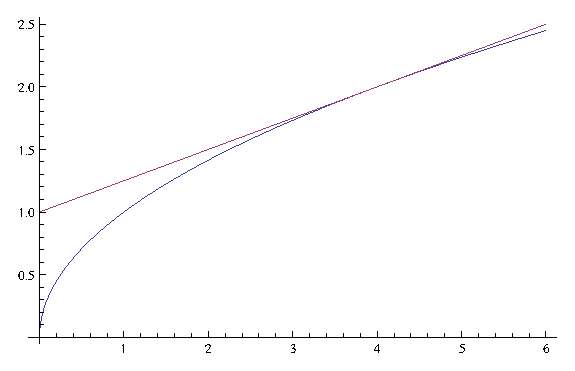
\includegraphics[width=0.5\textwidth]{continuous/derivatives/lin_ex1.eps}
      \end{center}
      \caption{A plot of $f(x)$ and $L_a(x)$.}
    \end{figure}
  \end{sol}
\end{ex}

\subsection{Graphing Functions}
To graph a function:\footnote{This section is copied from my notes from Dr. Dobrescu's Math 140 class, taken in Fall 2011 at Christopher Newport University.}
  \begin{enumerate}
   \item Find all \textbf{critical values}. Critical values are locations where $\frac{\ud y}{\ud x}=0$ or is undefined.\footnote{At locations where $\frac{\ud y}{\ud x}=0$, the tangent line is horizontal.}
   \item Find all \textbf{points of inflection}. These are locations where the second derivative ($\frac{\ud^2y}{\ud x}$) is zero or undefined.
   \item Determine where $\frac{\ud y}{\ud x}$ is \emph{positive} to find where $f(x)$ is \emph{increasing}. Remember that a derivative signifies the slope of a graph, so a positive derivative implies that the graph is increasing. This can be achieved either by testing values on each side of a \emph{critical value}, or by intuitive understanding. For example, $\frac{\ud y}{\ud x}=3x^2$ is positive everywhere except at $x=0$, so $f(x)=y$ is increasing everywhere except for at its horizontal tangent at $x=0$.\footnote{$x^2$ can never produce a negative number, because a negative times a negative or a positive times a positive is always positive}
   \item Determine where $\frac{\ud y}{\ud x}$ is \emph{negative} to find where $f(x)$ is \emph{decreasing}.
   \item Determine the sign of $\frac{\ud^2y}{\ud x}$ on both sides of all \emph{points of inflection}. The graph is \emph{concave up} where $\frac{\ud^2y}{\ud x}$ is positive, and \emph{concave down} where $\frac{\ud^2y}{\ud x}$ is negative.
  \end{enumerate}

\section{l'Hospital's Rule}\label{sec:lhospital}\index{l'Hospital's Rule}

\textbf{l'Hospital's Rule} uses derivatives to calculate limits\index{limits} of fractions whose numerators and denominators both approach the same indeterminate for, which can be either zero or $\infty$. Limits involving transcendental functions\index{transcendental functions} often require some use of the rule for their calculation.

\begin{theorem}[L'Hospital's Rule]\label{th:lhospital}
  Suppose that $f(a)=g(a)=0$, that $f$ and $g$ are differentiable on an open interval $I$ containing $a$, and that $g'(x) \neq 0$ on $I$ if $x \neq a$. Then
  \[ \lim_{x \to a} \frac {f(x)}{g(x)} \=H \lim_{x \to a} \frac{f'(x)}{g'(x)} \]
  assuming that the limit on the right side of this equation exists.
\end{theorem}
\begin{remark}
  L'Hopital's Rule does not apply when either the numerator or the denominator has a finite nonzero limit.
\end{remark}
The proof of this theorem is found in Section \ref{proof:lhospital}.
\begin{figure}[h]
  \begin{center}
    \includegraphics[width=0.2\textwidth]{photos/cauchy.jpg}
  \end{center}
  \caption{Augustin Louis Cauchy, 1901.}
\end{figure}
\begin{theorem}[Cauchy's Mean Value Theorem]\label{th:caunchymv}\index{Cauchy's Mean Value Theorem}
Suppose functions $f$ and $g$ are continuous on $[a, b]$ and differentiable throughout $(a, b)$ and also suppose $g'(x) \neq 0$ throughout $(a, b)$. Then there exists a number $c$ in $(a, b)$ at which
  \[ \frac {f'(c)}{g'(c)} = \frac{f(b)-f(a)}{g(b)-g(a)} \]
\end{theorem}
\section{Derivatives of Inverses of Differentiable Functions}\index{inverse
functions}

\begin{theorem}[The Derivative Rule for Inverses]\label{th:invderiv}
  If $f$ has an interval $I$ as domain and $f'(x)$ exists and is never zero on $I$, then $f^{-1}$ is differentiable at every point in its domain (the range of $f$). The value of $\big(f^{-1}\big)'$ at a point $b$ in the domain of $f^{-1}$ is the reciprocal of the value of $f'$ at the point $a=f^{-1}(b)$:
  \begin{equation}
    \big(f^{-1}\big)'(b)=\frac{1}{f'\big(f^{-1}(b)\big)}
  \end{equation}
  This can also be written
  \begin{equation}
    \cfrac{\ud f^{-1}}{\ud x}\bigg|_{x=b}=\cfrac{1}{\cfrac{\ud f}{\ud x}\bigg|_{x=f^{-1}(b)}}
  \end{equation}
  \begin{proof}
  Because a function applied to the inverse of itself should return its own input value, we can start with this relationship.
    \begin{align*}
      f \big( f^{-1}(x) \big) &= x \\
      \intertext{From here, take the derivative of both sides. On the left, we do so in notation only. On the right, we know that the derivative of a variable representing a constant is always 1.}
      \frac{\ud}{\ud x} f\big(f^{-1}(x)\big) &= 1\\
      \intertext{Because the lefthand side includes the composition of functions, we must use the chain rule in calculating its derivative. Applying the chain rule to the lefthand side of the equation gives us}
      f'\big(f^{-1}(x)\big)\cdot \cfrac{\ud}{\ud x}f^{-1}(x) &= 1  \\
      \intertext{Now, we divide each side of the equation by $f' \big( f^{-1}(x) \big)$ to solve for the derivative only.}
      \frac{\ud}{\ud x}f^{-1}(x) &= \cfrac{1}{f'\big(f^{-1}(x)\big)}\qedhere
    \end{align*}
  \end{proof}
\end{theorem}

\section{Antiderivatives}
\begin{defn}
  A function $F$ is an \textbf{antiderivative} of $f$ on an interval $I$ if $\forall (x \in I) \big[F'(x)=f(x)\big]$.
  \index{antiderivative}
\end{defn}
\begin{ex}
  Find an antiderivative of $f(x)=3x^2$.
  \begin{sol}
    We should think of a function whose derivative yields the function $3x^2$.
    It seems clear that this function is related to the power rule, and reversing that rule would give us $x^3$.
    Now let's take the derivative of this and see if it works.
    \begin{align*}
      F(x)&=x^3 \\
      F'(x) &= 3x^2
    \end{align*}
    What's interesting here is that $3x^2$ is not the only function for which its derivative is $3x^2$.
    We know from Theorem \ref{th:deriv:constantrule}, the constant rule for derivatives, that the derivative of any constant is zero.
    From this, we know that
    \[ F(x)=3x^2+1 \]
    or
    \[ F(x)=3x^2+20\]
    or even
    \[ F(x)=3x^2+39250\]
    all satisfy our definition for an antiderivative of $f(x)$.
    How do we write this?

    The \textbf{generalized antiderivative} of $f(x)$ is written
    \[ F(x)+c \]
    where $c$ is an ``arbitrary constant''--that is, any number whatsoever that does not contain a variable.
    This ``function,'' $F(x)+c$, therefore, does not actually refer to \emph{one} function in particular,
    or even a \emph{handful} thereof, but rather a \textbf{family of functions}, all of which have a derivative equal to $f(x)$.

    For our example, the generalized antiderivative of $f(x)=3x^2$ is $F(x)=x^3+c$.
  \end{sol}
\end{ex}
We would plot this using \textbf{integral curves}, which represent a variety of possible versions of the function for different values of $c$.
\begin{figure}[<+htpb+>]
  \begin{center}
    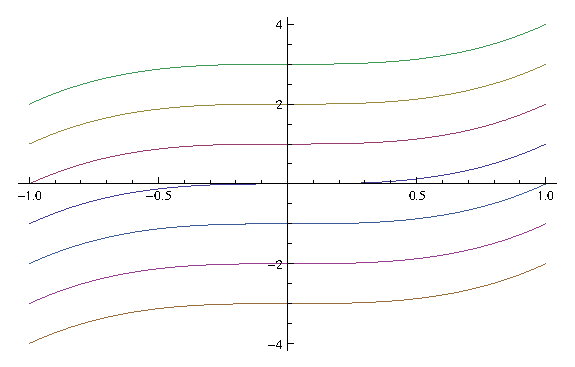
\includegraphics[width=3in]{continuous/derivatives/intcurves.eps}
  \end{center}
  \caption{A few possible integral curves for $F(x)=x^3+c$.}
\end{figure}
